\documentclass[12pt]{article}
\topmargin=0 in
\usepackage{amssymb}
\usepackage{pdfpages}

\title {Encrypting User Data with Attribute-Based Encryption Using Privacy Policies}
\author {Milo Watanabe \\ Boston College}
\date{April 2014}

\begin{document}

\maketitle

\begin{abstract}
As the internet and cloud services have pervaded our lives in nearly every aspect, one of the biggest issues facing the populace today is finding the best ways to protect our privacy. An important part of protection for the average user of a service is their privacy policy: essentially the only way today to let a client define how their data is used by the server. But often a client is not given a choice, and sometimes their policy is not even followed.
We present here an way of encrypting user data such that they first create a privacy policy, and their data is protected from even the service unless their privacy requirements are met by the service.
\end{abstract}

\section{Introduction}
Protecting user privacy is a huge problem facing any internet company, and a huge issue for every client using those technologies. Tech giants, like Facebook and Google, and smaller app developers, like QuizUp publisher Plain Vanilla, have faced a large amount of backlash based on their sometimes-shady usage of client data \cite{lawler}. More and more solutions are emerging for giving users finer control over their data, though. \\
Recently in the EU, a push has gone through the European Parliament to create tighter regulations for privacy and enforce larger penalties for noncompliance \cite{bajaj}. Another solution involves a new programming language that inherently puts constraints, defined by privacy policies, on certain variables that correspond to user data \cite{yang}. These are good solutions, and they are important steps towards putting the client first. One of the biggest issues with the current state of privacy, though, is that even if a user edits their privacy settings, often they are still left unclear as to how their data is managed, and frankly can't tell if it was mismanaged anyway. \\\\
The solution presented here will not go so far as to ensure the data is used properly, but it will create a `promise' that the service will implicitly make with every instance of the data being used. This scheme uses a type of Key-Policy encryption called Attribute-Based Encryption. It requires a client to share its data with a server, which will perform some action with the data, and a third-party authority to create and store the keys necessary for the data to be encrypted and decrypted. The prototype for such a system has been built as a web app called privateBook, in which clients create an account and set a privacy policy, then can write posts that they can view if signed in to their own account. This simple demonstration serves to show a practical way of ensuring data is encrypted for all parties, and can only be seen as a result of the service adhering to a user's privacy policy.

\section{Data Encryption}
At a high level, Attribute-Based Encryption (ABE) is a form of Public-Key cryptography which encrypts data with an access tree, or policy. A party attempting to decrypt the data must present an attribute list, which will successfully allow decryption provided the attributes satisfy the tree. We will discuss exactly how ABE uses policies and attributes to encrypt and decrypt data, and then how the privateBook implementation uses this type of encryption.

\subsection{Public-Key Cryptography}
In many systems of encryption there is one key that is used to encrypt and decrypt messages, called a cipher. This is analogous to one key that may lock or unlock a door. Public-Key cryptography is also called asymmetric cryptography, due to its use of two separate keys, one used to decrypt and one used to encrypt a message. In this form, there is both a public key and private key. The public key is used to encrypt data, while the private key is used to decrypt. The keys are generated with some function that creates a public key which does not allow a foreign party to discover the private key. This is based on certain problems which are essentially impossible to solve computationally, such as large integer factorization problems. 

\subsection{Attribute-Based Encryption}
The implementation of ABE is provided by Charm, a Python framework providing many different crypto systems \cite{charm}. There are four portions of the ABE scheme: the parameter setup, encryption, key generation, and decryption. 
\paragraph{Setup}
The setup simply generates random groups, which are stored as PK, the public parameters, and MK, the private key. PK is the ABE version of a public key. The two keys here are bilinear group generators raised to randomly chosen exponents. These are stored as Python dictionaries.
\paragraph{Encryption}
Encryption uses PK, $\gamma$, the access structure, along with the string message meant to be encrypted, $M$. A dictionary, $E$ is created, which is the encrypted cipher text. $\gamma$, a string of a boolean expression, is the policy that must be satisfied for decryption.
\paragraph{Key Generation}
Key Generation uses a list of attributes, $\mathbb{A}$, and MK to generate a decryption key, D. This is the ABE version of a private key, used to decrypt. $\mathbb{A}$ is the list of attributes that must satisfy $\gamma$ in order for D to successfully decrypt E. 
\paragraph{Decryption}
Decryption takes E, the ciphertext containing $\gamma$, PK and D. It applies D to E in order to decrypt the message. If $\mathbb{A}$ satisfies $\gamma$, in the sense of the attributes fulfilling the boolean expression included in D, the message will decrypt.

\subsection{Example Usage}
An example following the paper describing ABE's fine-grained access capabilities can demonstrate how this system would play out if used in exactly the way described above \cite{abe}. \\
If there were a system for storing activity logs on a network, this data would need to be protected by an encryption scheme that would vary for different types of information and different types of activity. Here, ABE encryption would be useful, as each log could be stored with a specific access policy: say "user is Bob or Alice AND the date is between September 2010 and May 2014 AND the activity is related to updating or changing the financial information of projects". This information would then be encrypted with this policy. Anyone investigating the logs could then be given a secret key with a specific access list with their properties: user name, title, security clearance, activity type, date, etc.  ABE would then only allow the analyst to access information if their information fit with the policy: all other data, which is not pertinent to their work, will be unaccessible.

\section{ABE Privacy Prototype}
The ABE prototype used here can apply to any service which uses client data to perform some function, whether it be like Facebook, just storing and displaying messages, text or multimedia, or something like Google Maps, which uses client location info to display a map or directions. In a sense, the prototype applies ABE in a backwards fashion: rather than encrypting with a policy, and users attempt to decrypt by presenting their attributes, here the attribute list is created and clients present their policies. Figure 1 displays the process. \\

\begin{center}
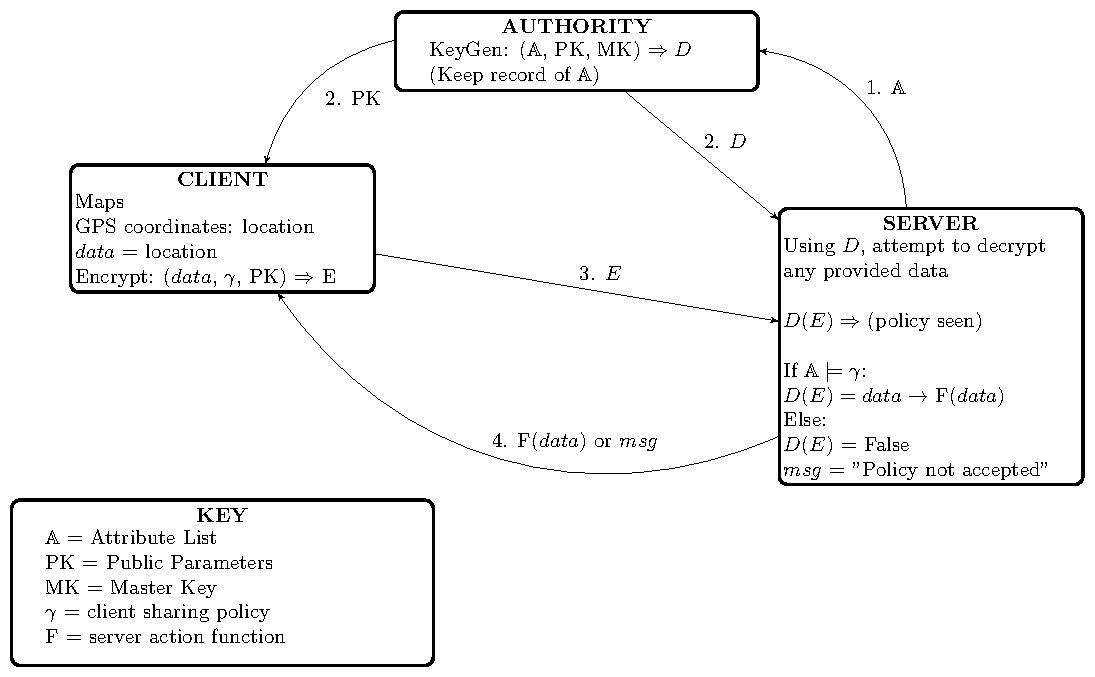
\includegraphics[scale=.7]{policydiagram.pdf} \\
\textbf{Figure 1: Prototype encryption/decryption process}
\end{center}

\subsection{Parties Involved}
In the prototype, there are three relevant parties involved: the server, which provides the service, a client, who uses the service, and the authority, a third party that creates, distributes and stores the keys for both parties. The server creates default settings for privacy, saving them as an attribute list. The client creates their own privacy settings, which is saved as a policy. The keys generated from these values are managed by an authority party. This is necessary as another layer of security for the client: if an authority generates the public and private keys, the client can be sure that the keys are generated properly. If a server generated the keys, they could possibly leave themselves a backdoor. The authority also would then have the ability to check the server's data use with their default privacy policy, and confirm that the server was truly using data in the way they had claimed. 

\subsection{The Full Process}
There are four steps of this scheme: server registration, key distribution, client encryption, and server response.

\paragraph{1. Server Registration}
This is the first step, and only happens once. The server registers with the Authority, naming itself and providing a list of attributes, $\mathbb{A}$, which is a list of the default values created for a privacy policy. The Authority stores $\mathbb{A}$.

\paragraph{2. Key Distribution}
This happens once, in three parts. The Authority generates PK and MK, the public parameters and master key, which are used to generate D. $\mathbb{A}$, PK and D are stored by the Authority. Then, D is sent to the server, which will use it to decrypt data, and PK is sent to the client, who uses it to encrypt data.

\paragraph{3. Client Encryption}
This will happen with every client request. The client encrypts by providing their data, $\gamma$, their personal privacy policy, and PK. This yields E, a cipher text, which is sent to the server. The server then stores the data as a cipher text.

\paragraph{4. Server Response}
This happens after every client request. The server stores the encrypted data, and attempts to decrypt it by applying the decryption key D to E. This will return either the original data or False. If $\mathbb{A}$ satisfies $\gamma$, the data will be properly decrypted, and the server can perform whatever functions it needs with the data and responds to the client indicating success. If the policy is not successfully satisfied by the attribute list, the server responds to the client indicating failure.

\section{privateBook}
The prototype of this scheme mimics an online diary: a user can make their own account, then write notes to themselves that will display on their page. The idea of using ABE is that, in decrypting the data, the server must know the privacy policy of the user presenting it. Thus successful decryption becomes analogous to an active promise that the service has read and will follow the user's wishes for privacy, rather than potentially ignoring a policy saved in some database. \\
There are three parts of the site: a server registration page, on which the server creates its attribute list and the Authority stores the keys and $\mathbb{A}$ in an Authority table, a client registration page, where a client creates his or her privacy policy, storing $\gamma$ and their identification information in a Policy table, and a homepage, where the client can write their updates and have them displayed; each update is stored by the server as a cipher text with a user ID in a Posted Data table. We will demonstrate each of the four steps in the privateBook implementation.

\subsection{privateBook Server Registration}
The privateBook server registers its name and default privacy settings with the Authority, which saves them as an attribute list, and then creates PK and D, the public parameters and private key. Figure 2 shows the printed values created from the default privateBook privacy values. \\ \\
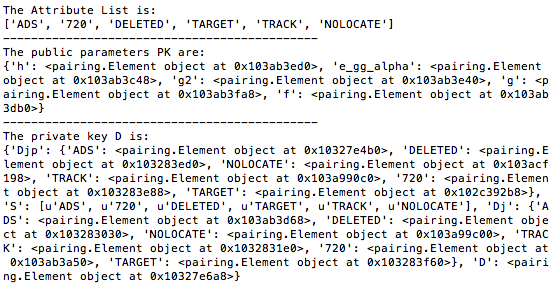
\includegraphics[scale=.705]{authority3.png}
\begin{center}
\textbf{Figure 2: Authority values (Attribute list, PK, D)}
\end{center}
These default values are based off the client privacy policy creation page, which is shown in Figure 3. \\
\begin{center}
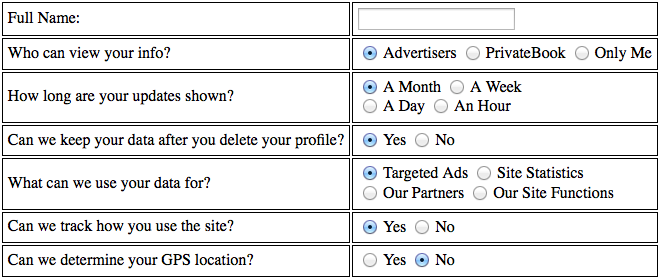
\includegraphics[scale=.55]{policycreation.png} \\
\textbf{Figure 3: Client Policy creation page}
\end{center}

\subsection{Authority Key Storage and Distribution}
The Authority then serializes the dictionary keys and stores them, shown in Figure 4. \\
\begin{center}
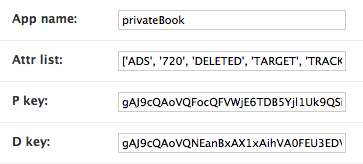
\includegraphics[scale=.9]{authoritydb.png} \\
\textbf{Figure 4: Authority key storage}
\end{center}
These keys are then provided to the server and the clients by way of database queries to the Authority table. In a real distributed system, the Authority would send back D to the server, which would store it on their own. The clients would then receive PK upon registering for the service, an added complexity that this prototype does not delve into. 

\subsection{Client Privacy Policy Creation}
The client, to become a privateBook user, registers themselves with a name and their privacy policy, as shown in Figure 3. They are then given their own ID, simply the order in which they were created, as their password, and username of their full name. These design choices are meant to simplify the account creation process: the focus of the prototype is not concerned with creating users as much as maintaining the privacy of their data, so privateBook has foregone security measures that should be in place in practical applications. Two policies are shown in Figure 5. They are strings of boolean expressions. The first is a policy that has the least privacy restrictions as given by the service, and the second has the strictest settings. The first includes an `or' for every type of privacy setting which includes all possible attributes; this allows for any default setting in the attributes list to satisfy the policy. The second, stricter policy includes the fewest attributes, making it the most difficult to satisfy.

\begin{center}
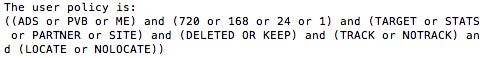
\includegraphics[scale=.8]{policy.png} \\
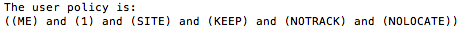
\includegraphics[scale=.85]{policy2.png} \\
\textbf{Figure 5: Least strict and most strict user privacy policies}
\end{center}
This method of creating a default attribute list was to allow the server to fail. In practice, a service that intends to have wide use should never fail, and thus an early idea was to simply let each attribute be the type of privacy setting it was, and store the values elsewhere. Then the server would still need to decrypt the data and thus inherently read the privacy policy, but that would offer no real difference from what exists currently, as the actual privacy settings would still be stored somewhere and potentially ignored, as they are now. So a difficulty arose in finding an appropriate method to allow one attribute list to successfully satisfy many different policies. This method was chosen because it is based on an idea of having different levels of privacy, where a baseline is chosen by the service and clients can be more or less strict; more, rendering the service useless for that user, and less, allowing for full use.

\subsection{Client Encryption and privateBook Response}
The client then makes a status update, much like a Facebook one, and submits that. The data is encrypted with the update, a string, along with the user's privacy policy and the public key PK. This results in a long cipher text, which is stored in privateBook's database as a serialized dictionary. The results of this process are shown in Figure 6. E is stored in the database, then the page is reloaded, displaying all of the user's updates. The server, upon loading of the user's homepage, first attempts to decrypt their data. If it is successful, the date, time and actual content are shown. If it is unsuccessful, the content is replaced with: ``Your status could not be displayed: this service does not support your privacy policy!" Thus this service will not work for the client if their privacy settings are too strict, and therefore their policy is not satisfied by privateBook's default attribute list. 

\begin{center}
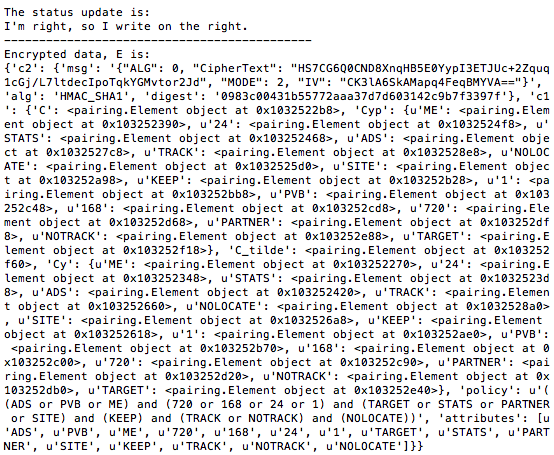
\includegraphics[scale=.65]{posteddata.png} \\
\textbf{Figure 6: The plaintext update and it's corresponding encrypted cipher text}
\end{center}

\section{Issues with the Prototype}
Though the privateBook prototype offers a solution, there are, as can be expected, some faults. The biggest issue is that the encrypted data, E, is extremely large. As all large internet services have constraints on their memory already, and must constantly work towards improving memory efficiency, this solution definitely puts consumer needs before those of the service, to put it lightly. A fix for that problem could involve compression of the encrypted data, but this would put a large amount of strain on the backend and undeniably cause slower speeds of service, another big concern for internet companies. \\
Another catch to this system is that it still does not solve the issue of misuse of data. Though it forces companies to actively accept user privacy policies, it does nothing to enforce them. This responsibility would most likely fall to the Authority, which would need to have access to an enormous amount of data and track its use, which in itself could be considered contradictory to the original purpose of the scheme. 

\section{Conclusion}
The privateBook prototype demonstrates a possible use of ABE encryption in protecting user privacy, which can be considered an important step in a controversial yet important problem. Though this implementation is far from perfect, it offers a unique solution: using the current model of a privacy policy, and extending it to giving users actual control over how the company using their data, at minimum, claims to use it. This solution calls for better legislation and improved memory storage options, but hopefully can take its place as one part of a series of improvements aimed at better protection for users of internet services. \\ \\ \\ \\ \\ \\ \\ \\

\renewcommand{\abstractname}{Acknowledgements}
\begin{abstract}
 Professor Robert Muller and Stefan Saroiu at Microsoft Research
\end{abstract}

\begin{thebibliography}{9}

\bibitem{lawler}
Lawler, Ryan. "QuizUp Sends Personal User Info To Strangers, Company Says Bug Contributed To Weakened Security." TechCrunch, 25 Nov. 2013.
\bibitem{bajaj}
Bajaj, Vikas. "Imagine if Companies Had to Ask Before Using Your Data." Taking Note. The New York Times, 13 Mar 2014.
\bibitem{yang}
J. Yang, K. Yessenov, A. Solar-Lezama. A Language for Automatically Enforcing Privacy Policies. \textit{POPL} 2012.
\bibitem{charm}
Akinyele, Joseph A. and Garman, Christina and Miers, Ian and Pagano. ``Charm: a framework for rapidly prototyping cryptosystems." \textit{Journal of Cryptographic Engineering} 3.2 (2013): 111-128.
\bibitem{abe}
J. Bethencourt, A. Sahai, B. Waters. Ciphertext-Policy Attribute-Based Encryption.
\end{thebibliography}
















\end{document}